%%


%% This is file `sample-manuscript.tex',
%% generated with the docstrip utility.
%%
%% The original source files were:
%%
%% samples.dtx  (with options: `all,proceedings,bibtex,manuscript')
%% 

%%
%%
%% Commands for TeXCount
%TC:macro \cite [option:text,text]
%TC:macro \citep [option:text,text]
%TC:macro \citet [option:text,text]
%TC:envir table 0 1
%TC:envir table* 0 1
%TC:envir tabular [ignore] word
%TC:envir displaymath 0 word
%TC:envir math 0 word
%TC:envir comment 0 0
%%
%% The first command in your LaTeX source must be the \documentclass
%% command.
%%
%% For submission and review of your manuscript please change the
%% command to \documentclass[manuscript, screen, review]{acmart}.
%%
%% When submitting camera ready or to TAPS, please change the command
%% to \documentclass[sigconf]{acmart} or whichever template is required
%% for your publication.
%%
%%
\documentclass[manuscript,screen,review]{acmart}
\usepackage{subfigure}
\usepackage[normalem]{ulem}
\usepackage{booktabs}
\usepackage{csquotes}
\usepackage{siunitx}
\usepackage{fancybox}
\usepackage[acronym]{glossaries}
\usepackage[inline]{enumitem}
\makeglossaries
\glsdisablehyper

\newacronym{sip}{SIP}{Stereo Image Profile}
\newacronym{vr}{VR}{Virtual Reality}
\newacronym{ar}{AR}{Augmented Reality}
\newacronym{xr}{XR}{Extended Reality}
\newacronym{srm}{SRM}{Spatial Release from Masking}
\newacronym{mushra}{MUSHRA}{MUltiple Stimuli with Hidden Reference and Anchor}
\newacronym{hrir}{HRIR}{Head-Related Impulse Response}
\newacronym{hints}{HINTS}{Human-Centered Intelligent Realities}
\newacronym{asa}{ASA}{Auditory Scene Analysis}
\newacronym{msa}{MSA}{Musical Scene Analysis}
\newacronym{tts}{TTS}{Text-to-Speech}

%%
%% \BibTeX command to typeset BibTeX logo in the docs
\AtBeginDocument{%
  \providecommand\BibTeX{{%
    Bib\TeX}}}

%% Rights management information.  This information is sent to you
%% when you complete the rights form.  These commands have SAMPLE
%% values in them; it is your responsibility as an author to replace
%% the commands and values with those provided to you when you
%% complete the rights form.
\setcopyright{acmlicensed}
\copyrightyear{2025}
\acmYear{2025}
\acmDOI{XXXXXXX.XXXXXXX}
%% These commands are for a PROCEEDINGS abstract or paper.
%\acmConference[Conference acronym 'XX]{Make sure to enter the correct
%  conference title from your rights confirmation email}{June 03--05,
%  2025}{Woodstock, NY}
%%
%%  Uncomment \acmBooktitle if the title of the proceedings is different
%%  from ``Proceedings of ...''!
%%
%\acmBooktitle{Woodstock '18: ACM Symposium on Neural Gaze Detection,
%%  June 03--05, 2018, Woodstock, NY}
% \acmISBN{978-1-4503-XXXX-X/2018/06}


%%
%% Submission ID.
%% Use this when submitting an article to a sponsored event. You'll
%% receive a unique submission ID from the organizers
%% of the event, and this ID should be used as the parameter to this command.
%%\acmSubmissionID{123-A56-BU3}

%%
%% For managing citations, it is recommended to use bibliography
%% files in BibTeX format.
%%
%% You can then either use BibTeX with the ACM-Reference-Format style,
%% or BibLaTeX with the acmnumeric or acmauthoryear sytles, that include
%% support for advanced citation of software artefact from the
%% biblatex-software package, also separately available on CTAN.
%%
%% Look at the sample-*-biblatex.tex files for templates showcasing
%% the biblatex styles.
%%

%%
%% The majority of ACM publications use numbered citations and
%% references.  The command \citestyle{authoryear} switches to the
%% "author year" style.
%%
%% If you are preparing content for an event
%% sponsored by ACM SIGGRAPH, you must use the "author year" style of
%% citations and references.
%% Uncommenting
%% the next command will enable that style.
%%\citestyle{acmauthoryear}


%%
%% end of the preamble, start of the body of the document source.
\begin{document}

%%
%% The "title" command has an optional parameter,
%% allowing the author to define a "short title" to be used in page headers.
\title{Perceptual Evaluation of Binaurally Panned Speech and Music Mixtures}

%%
%% The "author" command and its associated commands are used to define
%% the authors and their affiliations.
%% Of note is the shared affiliation of the first two authors, and the
%% "authornote" and "authornotemark" commands
%% used to denote shared contribution to the research.

%
\author{Richard Mitic}
\authornote{These authors contributed equally and share first authorship.}
\orcid{0000-0003-3232-191X}
\affiliation{%
  \institution{School of Innovation, Design and Engineering, Mälardalens Universitetet}
  \city{Stockholm}
  \country{Sweden}}
\email{richard.mitic@mdu.se}
%

\author{Majed Elwardy}
\authornotemark[1]
\orcid{0000-0002-7550-5818}
\affiliation{%
  \institution{Department of Computer Science, Blekinge Institute of Technology}
  \city{Karlskrona}
  \country{Sweden} }
\email{majed.elwardy@bth.se}
%
%
\author{Veronica Sundstedt}
\orcid{0000-0003-3639-9327}
\affiliation{%
  \institution{Department of Computer Science, Blekinge Institute of Technology}
  \city{Karlskrona}
  \country{Sweden}
}
\email{veronica.sundstedt@bth.se}
%
%
\author{Andreas Rossholm}
\orcid{0009-0001-5678-038X}
\affiliation{%
 \institution{Media Quality Lab, Spotify AB}
 \city{Stockholm}
\country{Sweden}
}
\email{arossholm@spotify.com}

%
%
\author{Yan Hu}
\orcid{0000-0002-3283-2819}
\affiliation{%
  \institution{Department of Computer Science, Blekinge Institute of Technology}
  \city{Karlskrona}
  \country{Sweden} }
\email{yan.hu@bth.se}


%
%
%%
%% By default, the full list of authors will be used in the page
%% headers. Often, this list is too long, and will overlap
%% other information printed in the page headers. This command allows
%% the author to define a more concise list
%% of authors' names for this purpose.
\renewcommand{\shortauthors}{Mitic et al.}

%%
%% The abstract is a short summary of the work to be presented in the
%% article.
\begin{abstract}
Music streaming services have the opportunity to adapt the listening experience for each user. This can include the option of interspersing speech audio with music tracks, providing interesting information to the listener. It is also possible to mix speech audio with music, although there is a lack of research which studies the most effective ways to achieve a pleasant listening experience. This paper describes a subjective test in which volunteer participants were asked to rate the pleasantness of music mixed with relevant speech. The speech signal was panned binaurally between 45\textdegree~left and 45\textdegree~right, in 15\textdegree~ increments, and mixed with various music tracks at equal loudness, with the hypothesis that this would improve the pleasantness ratings compared to centrally panned speech. The results indicate that the centre is not always the optimum panning position, and future work should investigate potential links between panning angle and musical features.
\end{abstract}

%%
%% The code below is generated by the tool at http://dl.acm.org/ccs.cfm.
%% Please copy and paste the code instead of the example below.
%%
\begin{CCSXML}
<ccs2012>
   <concept>
       <concept_id>10003120.10003121.10003122.10003334</concept_id>
       <concept_desc>Human-centred computing~User studies</concept_desc>
       <concept_significance>500</concept_significance>
       </concept>
   <concept>
       <concept_id>10010405.10010469.10010475</concept_id>
       <concept_desc>Applied computing~Sound and music computing</concept_desc>
       <concept_significance>500</concept_significance>
       </concept>
   <concept>
       <concept_id>10002951.10003227.10003251.10003255</concept_id>
       <concept_desc>Information systems~Multimedia streaming</concept_desc>
       <concept_significance>500</concept_significance>
       </concept>
 </ccs2012>
\end{CCSXML}

\ccsdesc[500]{Human-centred computing~User studies}
\ccsdesc[500]{Applied computing~Sound and music computing}
\ccsdesc[500]{Information systems~Multimedia streaming}

%%
%% Keywords. The author(s) should pick words that accurately describe
%% the work being presented. Separate the keywords with commas.
\keywords{Music, Speech, Music Mixtures, Binaural panning, User study, Subjective test, Perceptual evaluation}

\received{15 October 2025}
\received[revised]{-}
\received[accepted]{-}

%%
%% This command processes the author and affiliation and title
%% information and builds the first part of the formatted document.
\maketitle

\section{Introduction}
%This document is a model and instructions for \LaTeX. Please observe the conference page limits
% {\color{red} Richard/Andreas - something on the increase of streaming and importance of personalization?} 

The rise of music streaming services in recent years has provided users with listening experiences on multiple levels, and personalized experiences have been identified as a rising factor in the adoption of these services~\cite{barata_music_2021}. When personalization is mentioned, it generally refers to recommending tracks or playlists that a user might like. However, more recently, other areas, such as personalized user interfaces, have also emerged~\cite{noauthor_ai_2024}. In parallel, high-quality text-to-speech services have become much more readily available, to the point where they can be used to generate personalized informational audio about the music, for example, as in \cite{noauthor_spotify_2023}. One option for adding speech to music is to intersperse the two. However, in the realm of \gls{ar}, it is normal to overlay speech on top of background sounds. 

% In addition, in recent years, music streaming services have begun to use generative AI (GenAI) to provide additional information about the music being listened to in the form of voice. One example is Spotify's "AI DJ" feature, which uses synthesized voices to explain and elaborate on upcoming song recommendations and provide short interjections between tracks~\cite{noauthor_spotify_2023}. It is notable that in this example, voice and music are played sequentially, and they are never heard simultaneously. However, in the realm of Augmented Reality (AR), it is normal to overlay speech on top of background sounds. 

% {\color{red} Richard/Andreas - something more on AI DJ, be more specific about one voice, which one it is, limitations?} 

Although all of these technologies have begun to emerge, further research is needed to determine how speech and music should be presented to listeners and to identify user preferences. For example, it is known that mixing music or acoustic noise with speech results in a drop in intelligibility and perceived quality of the speech itself~\cite{fichna2022}. However, there is currently little research on how music and speech can be mixed acceptably and pleasantly. Unexplored variables include the spatial location of the speech, the gender of the voice, and the relative loudness of the music and speech.

This paper describes a perceptual evaluation designed to investigate how the panning position of speech audio mixed with music influences the perceived pleasantness of the mixture as a whole. Speech audio was binaurally panning between 45\textdegree~left and 45\textdegree~right in 15\textdegree~increments, and overlaid with a range of music tracks.

The remainder of the paper is organized as follows. Section~\ref{Background} describes the relevant concepts for the study, and Section~\ref{RelatedWork} presents related work. The method describing the experiment is presented in Section~\ref{Method}, and the results are analysed and discussed in Section~\ref{sec:ResultsAnalysis}. Finally, the work is concluded, and future work is suggested in Section~\ref{Conclusions}.

\section{Background}\label{Background}
%Andreas/Richard:
%Key terms and concepts
\gls{srm} is a well-studied phenomenon in which humans can perceive more detail in two sounds that come from different directions than if they come from the same direction. The associated research problem is \enquote{The cocktail party effect}, which refers to the problem of perceiving speech in the presence of other interfering noises \cite{litovsky_spatial_2012}.

Binaural panning is an advanced audio spatialization technique in which a monophonic signal is modelled as a point source at a specific angle from the listener's ears. It can be achieved by convolving the mono signal with the left and right \gls{hrir} recorded from binaural microphones. Headphones are typically required to hear the correct effects of binaural panning. It differs from amplitude panning, in which the amplitude of a signal is adjusted in the left and right channels to make the audio source appear to come from a different direction. Amplitude panning is common in music production, whereas binaural panning is typically used more in \gls{vr}, \gls{ar}, and \gls{xr}.

\gls{sip} refers to a description of the stereo field in an audio recording. There are multiple types of \gls{sip}, some of which are summarized in~\cite{mitic_towards_2025}, which recommends modifying the existing types to fit a specific task. One such \gls{sip} is \enquote{Panning Histogram}~\cite{gomez_music_2008}, which describes the likelihood that a stereo audio signal has energy at a given azimuth position (and optionally in a given frequency band). Notably, the \enquote{panning azimuth} is a dimensionless value that spans from left to right.



\section{Related Work}
\label{RelatedWork}
The clarity and intelligibility of speech when masked with another sound source have been major research topics for decades. One particular area of interest is speech in reverberant environments, with research dating back to the 1950s~\cite{muncey1953acceptability}, and continuing to this day.

A second broad area of speech intelligibility research is related to the effects of interference noise. This can take the form of other speakers, environmental noise, artificial noise, and (more recently) music. For example, the second Clarity Enhancement Challenge (CEC2) introduced music as an interfering source only in 2023~\cite{akeroyd_2nd_2023}. The music in question was synthesized as a point source at a fixed distance from the artificial listener. Similarly,~\cite{fichna_perceptual_2022} used a single musical instrument as a masking sound when testing speech intelligibility in a \gls{vr} environment.

In the vast majority of research in this field, the intention was to reveal or enhance a speech signal to increase its intelligibility. However, the authors have not found previous research on the subjective opinions of music combined with relevant speech, a gap that this perceptual evaluation aims to fill. In fact,~\cite{madsen_music_2014} found that simple subjective tests on the perceptual quality of music had been largely neglected in hearing aid research. 

A recent study on \gls{asa} and \gls{msa} concluded that a subject's age has a moderate effect on their ability to organise complex auditory mixtures into meaningful events~\cite{hake_individual_2025}. This study used separate tasks to assess \gls{asa} for speech and \gls{msa} for music, and did not attempt to mix the two. In a similar vein,~\cite{benjamin_evaluating_2024} collected both subjective ratings of manipulated music and \gls{msa} scores, concluding that better subjective ratings correlated with higher \gls{msa} scores for younger, normal-hearing listeners.

%{\color{blue}
% Subjective audio quality assessment is a technique used to evaluate Audio Quality (AQ). With the rise of immersive multimedia, it is essential to integrate human behaviour, considering how people naturally interact with spatial sound~\cite{Smimite_2014}. Recently, several studies have focused on assessing spatial audio. In~\cite{berg2003}, the AQ assessment for spatial attributes was performed using only verbal expressions, which inevitably leads to biased results (explain more). In~\cite{LeBagousse_2012}, spatial audio was assessed with three families of attributes, such as timbre, space, and defects.  

% TBC...

% This paper discusses the relationship between classical music composers from different periods, such as the classical, romantic, and 20th-century periods, and their performances connected to spatial sound~\cite{Cihan_2020}.


% In this work, AudioMiXR, an AR interface intended to assess how users manipulate virtual audio objects situated in their physical space using six degrees of freedom (6DoF), is deployed on a head-mounted display (Apple Vision Pro) for 3D sound design. This work shows the first 6DoF AR interface for sound design, enabling direct free-hand manipulation of spatial audio. The results suggest that the embrace of 6DoF in XR audio mixing has distinct features that enhance the user experience for 3D audio mixing in contexts where the involvement of the body or free range of motion is beneficial for different applications, such as XR applications, music, where audio mixing with 6DoF in AR-VR may benefit~\cite{woodard2025}.

% This paper proposes a system for spatial audio generation that integrates visual components, including object detection, depth estimation, and audio spatialization. The system aimed to simplify the transformation of mono-audio into binaural audio in multi-speaker scenarios without relying on a binaural dataset. The results demonstrate that the method significantly improves spatial consistency between audio and video, enhances speech quality, and performs robustly in multi-speaker scenarios~\cite{liu2025visual}.

% In recent years, many studies have focused on audio quality in
% spatial sound systems based on subjective tests, in which
% assessors grant a quality score. In addition, studies are using sensors to identify gestures to obtain more accurate results [A New Approach for Spatial Audio Quality Assessment]

%}


\section{Method}\label{Method}
%Veronica/Yan:

This project aims to explore the subjective evaluation of spatialized speech in music. Data were collected using rankings and questionnaires. The test procedure follows a \acrshort{mushra}-like structure.

\subsection{Setup}
The experiment was conducted in a controlled laboratory environment, free from external disturbances. During the experiment, participants were comfortably seated on a soft chair. A Mac laptop was used to display the experiment stimuli, which consisted of a graphical interface, as shown in Figure~\ref{interface}. A pair of Sennheiser HD 650 headphones was used together with a Focusrite Scarlett Solo 3rd Gen, to allow each participant to modify the volume to a suitable setting, as permitted by~\cite{itu-r-bs-1534_MUSHRA}.

\subsection{Participants}

A subjective test was conducted with 29 participants, comprising 22 males, six females, and one participant who preferred not to disclose their gender. Age data were available for 28 participants, ranging from 20 to 60 years, with a mean age of 36.61 years and a standard deviation of 10.02. Generally, participants who were over 18 years of age and had no hearing impairment were invited to participate in the study. Before participating, they received an information letter with detailed instructions on the experiment. In the laboratory, the participants were always accompanied by a researcher conducting the study. If necessary, further details were explained to them upon their arrival at the laboratory. 

During the experiment, the participant would listen to audio on commercial headphones. No risk was foreseen to the participant, and they were informed in advance that the experiment could be terminated at any point without giving a justification. If they volunteered to participate, they signed a consent form that was kept separate from any data collected through rankings and questionnaires. There was no reward for participating in the experiment. After informed consent, demographic information and experience with streaming services were collected using a questionnaire with a randomized identification number. 

\subsection{Audio Stimuli}
\label{subsec:audio_stimuli}
All audio stimuli consisted of a commercially recorded music track combined with a speech recording. The speech recordings were generated using a commercial \gls{tts} service, with the text being extracted from the Wikipedia~\cite{wikipedia} page of the track's primary artist. To balance the gender of the speech voice, 50\% of the tracks were assigned a male \gls{tts} voice and 50\% a female \gls{tts} voice. The mono speech recording with no music was used as the reference signal for each track. 

Each variant of a track was created by applying binaural panning of the speech signal at angles \{45L, 30L, 15L, 0, 15R, 30R, 45R\} (where L and R denote left and right, and the number denotes the panning azimuth in degrees from the centre line), as shown in Figure~\ref{binauralPanning}. Binaural panning was achieved by convolving the mono speech signal with the left and right \glspl{hrir} recorded by binaural microphones on the KEMAR dummy head subject of the SADIE II database~\cite{armstrong_perceptual_2018}. This database of \glspl{hrir} contains a set in which the excitation sound came from the exact angles specified; no interpolation of the \gls{hrir} coefficients was performed. A block diagram for a single azimuth is shown in Figure~\ref{stimulusCreation}, in which thin solid lines represent mono signals, thick solid lines represent stereo signals, and dotted lines represent duration metadata. The \enquote{Upmix} block represents a simple mono-to-stereo process whereby a mono recording is copied into both the left and right channels. The \enquote{Trim} block represents a process where the music excerpt is truncated to match the length of the binaurally panned speech. The \enquote{Normalize loudness} blocks represent changes in audio gain to ensure that the resulting loudnesses of both speech and music were equal.

\begin{figure}[tbp]
\centering
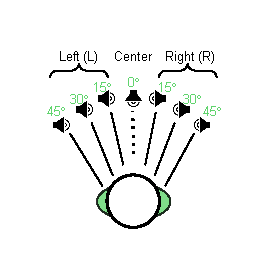
\includegraphics[trim=0.6cm 0.7cm 0.6cm 0.6cm, clip=true,width=0.35\columnwidth]{speech_angles.pdf}
\caption{The binaural panning of the speech signal at the different angles.}
\label{binauralPanning}
\end{figure}

\begin{figure}[tbp]
\centering
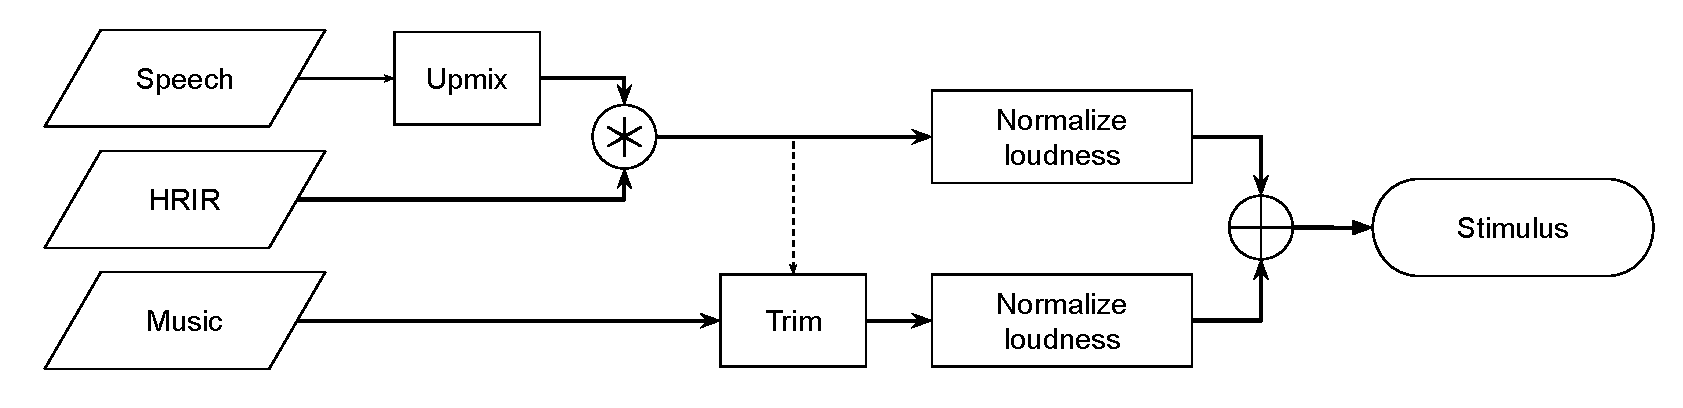
\includegraphics[width=0.9\columnwidth]{binaural_stimulus_creation.pdf}
\caption{Block diagram of the audio stimulus creation process for a single azimuth.}
\label{stimulusCreation}
\end{figure}

Once the binaurally panned speech signal was created, an excerpt of the music track was selected to be (1) musically representative of the track as a whole and (2) precisely the same length as the speech signal. The method of finding a representative section is detailed in \cite{jehan_extracting_2018}. The speech and music signals were then normalized to the same loudness using the pyloudnorm library \cite{steinmetz_pyloudnorm_2021} (which is an implementation of the ITU-R BS.1770 standard \cite{itu-r-bs-1770_lufs}) and summed to produce the final audio stimuli. In total, six different music tracks were selected, each combined with a different speech recording. The speech recordings were generated using both male and female voices, with three recordings featuring male voices and three featuring female voices. Table \ref{musicspeech} summarizes the music tracks, their corresponding speech recordings, and the gender of the voices used.
\renewcommand{\arraystretch}{1.2}
\begin{table}[h]
\centering
\setlength\tabcolsep{5pt}
\begin{tabular}{lll}
\toprule
 \textbf{Music Track} & \textbf{Speech Track} & \textbf{Voice Gender}\\        
\midrule
 Brown Eyed Girl & Van Morrison & Female\\
 Everyday Is A Winding Road & Sheryl Crow & Male\\
 Fake Plastic Trees & Radiohead & Female\\
 Fly Me To The Moon & Frank Sinatra & Male\\
 World In My Eyes & Depeche Mode & Male\\
 bad guy & Billie Eilish & Female\\
\bottomrule
\end{tabular}
\caption{The music tracks, along with their corresponding speech recordings and the gender of the voices.}
\label{musicspeech}
\end{table}


\subsection{Procedure and Experiment Interface}
In the experiment, participants could first adjust the volume to a comfortable level for themselves~\cite{itu-r-bs-1534_MUSHRA}. The application then presented the interface, shown in Figure~\ref{interface}, to familiarize them with the experimental procedures and different equipment. This was done before the formal experiment, which involved listening to and rating various audio clips. Each session lasted a maximum of 30 minutes.

Before the start of the experiment, participants were asked four questions: (1) How old are you?, (2) What is your gender? (Male/Female/Other/Prefer not to say), (3) How often do you use streaming services to listen to the following? Music streaming (A. Never use/B. Daily/C. Weekly/D. Monthly), How many hours do you listen to B/C/D?, Podcast (A. Never use/B. Daily/C. Weekly/D. Monthly), How many hours do you listen to B/C/D?, and (4) Do you consider yourself an expert listener? (A. Yes/B. No/C. I do not know).

The listening section of the test is closely based on the \gls{mushra} standard~\cite{itu-r-bs-1534_MUSHRA}. Participants are presented with a reference signal along with several variants and are asked to rate each based on how pleasant it is to listen to compared to the reference. The ranking scale follows the \gls{mushra} standard in that the opinion is a numeric value between 0 and 100, with the scale split into five equal sections marked by the words \enquote{Excellent}, \enquote{Good}, \enquote{Fair}, \enquote{Poor}, and \enquote{Bad}. Both the order of the variants and the order of the tracks are randomized for each subject, and the names of the variants are replaced with anonymized versions (see Figure~\ref{interface}). The test procedure differs from \gls{mushra} in that the variants for each track do not contain a hidden reference or hidden anchor. This is because the subjects were not asked to evaluate a signal degradation but rather a new signal assumed to be more pleasant than the reference. The information collected by the test interface comprised the ratings given to each variant.

After the experiment, participants were asked to complete a questionnaire about their listening experience. In particular, they were asked:
\begin{enumerate*}
    \item Can you justify what influenced your ranking of spatialized voice in music? (with a free-text answer)
    \item Do you prefer female or male voice in music? (A. Female voice, B. Male voice, C. No difference, or D. I do not know)
    \item What did you think about the relationship between the volume of voice and music? (A. The voice was: too quiet, good, too loud, B. The music was: too quiet, good, too loud).
    \item Do you have any further feedback on the experiment? (with a free-text answer).
\end{enumerate*}

The experiment interface, in Figure~\ref{interface}, presented the participant with (for each track) a waveform display depicting the track, the track title, the artist name, a set of vertical sliders to give their rating of each variant, and a play/pause button for each variant in addition to the reference. When audio is playing, it is looped, and the waveform display can be used to set the loop points.

\begin{figure}[ht]
\centerline{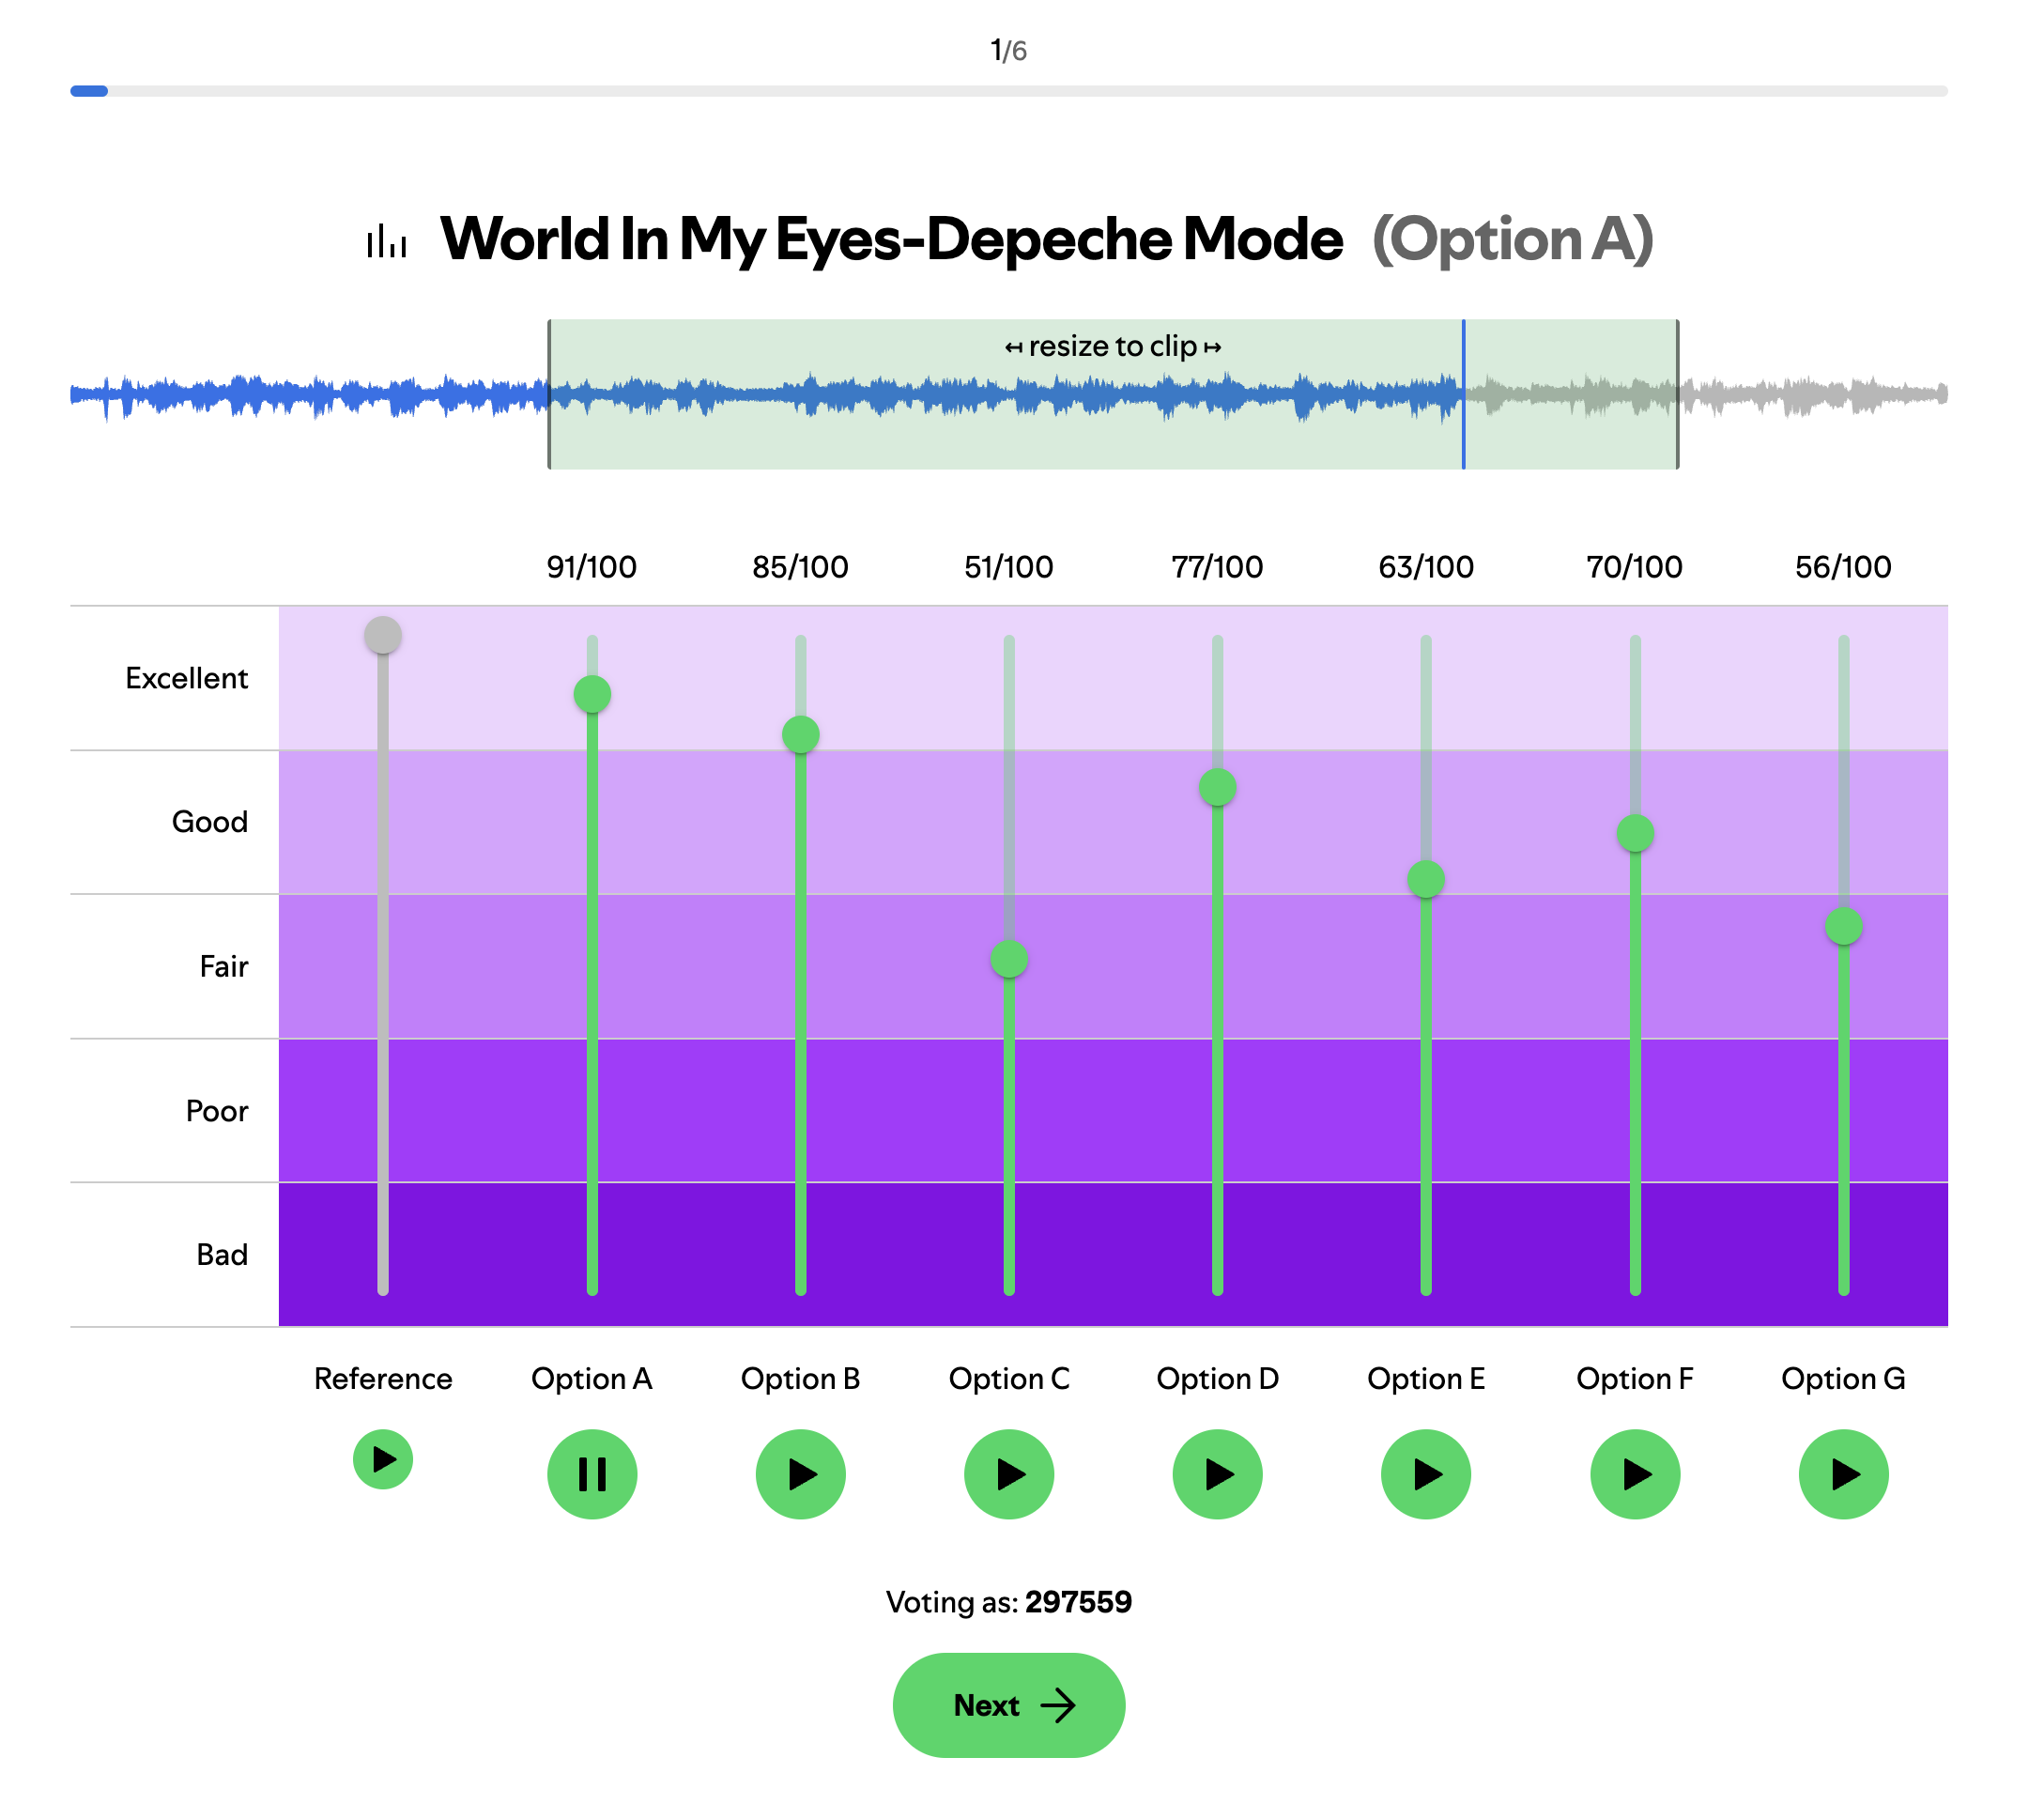
\includegraphics[width=0.65\textwidth]{screenshot_cropped.png}}
\caption{The experiment interface used in the perceptual evaluation.}
\label{interface}
\end{figure}

\section{Results and Analysis}
\label{sec:ResultsAnalysis}

Before the test, the participants were informed that a higher score indicated a greater pleasantness, but were given only basic instructions regarding the exact value of the score. Therefore, in the analysis, we assume that the scores are ordinal but with unequal intervals, and hence we only use statistical tests on the ranks of the scores. Ranks are calculated per-person-per-track. 

\subsection{Comparison of Centre to Non-Centre Preference}
\label{sec:noncentrepref}

In Section \ref{subsec:audio_stimuli}, it was established that the reference signal was a monophonic speech recording. It is standard practice that, by default, a monophonic audio signal is placed exactly in the centre of a stereo rendering. The perceptual evaluation, therefore, assesses whether the test participants gave any preference to the non-centred variants of panned speech. To do this, a Boolean variable was assigned denoting whether the top choice was centre or non-centre. If there was a tie, the centre won. This new dataset comprises a list of 174 preferences (29 participants $\times$ 6 tracks).

A ratio $R$ representing the proportion of non-centre preference was calculated by $S/N$ where $S$ is the number of results indicating a non-centre preference and $N$ is the total number of results. These values are presented in Table~\ref{table:ratios}, both for the entire dataset and for each music track. Subsequently, these ratios are tested against two null hypotheses using a binomial test. The null hypotheses ($H_0$) and their associated alternative hypotheses ($H_a$) are given in Table~\ref{table:hypotheses}. 


\begin{table}[h]
\centering
\begin{tabular}{llll}
\toprule
& $H_0$ & $H_a$ & Explanation of $H_0$ \\
\midrule
(1) & $R=0$ & $R>0$ & The centre variant was always preferred \\
(2) & $R=\frac{6}{7}$ & $R\neq\frac{6}{7}$ & The participants chose randomly \\
\bottomrule
\end{tabular}
\caption{Null hypotheses that the results were tested against.}
\label{table:hypotheses}
\end{table}

Table~\ref{table:ratios} shows the resulting p-values from the binomial test. Assuming a 95\% confidence interval, it can be seen that, with one exception (circled), all null hypotheses can be rejected. The exception is the track \enquote{Fake Plastic Trees}, for which the second null hypothesis (the test participants chose randomly) cannot be rejected. It can therefore be concluded that (for all other tracks) the default, centre-panned voiceover was not universally preferred.

Further tests were performed to determine whether there was any difference between other groupings. The complete dataset was stratified by voiceover gender, participant's age, music streaming usage, podcast usage, and expert listener status. Contingency tables were constructed with the independent variable being the different values of the strata and the dependent variable being the participants' centre/non-centre preference. Chi-square ($\chi^2$) tests were performed on the contingency tables with the null hypothesis that the grouping was independent of preference. For all groupings, the $\chi^2$ statistic was below the critical value and the p-value was above 0.05 (95\% confidence) and therefore the null hypotheses could not be rejected. Thus, all the variables tested were deemed independent of centre / non-centre preference. %The complete results are shown in Appendix~\ref{app:centre_preference_full}. 

%(the numbers comes from the distribution we have in the figures, it took the figures away but in that case we may have it in appendix .. we discuss.


\begin{table}[h!]
\centering
\begin{tabular}{lccccc}
\toprule
Group & $S$ & $N$ & $R$ & P-value $H_{0(1)}$ & P-value $H_{0(2)}$ \\
\midrule
All & 103 & 174 & \num{0.59} & \num{1.37e-42} & \num{1.27e-17} \\
Brown Eyed Girl - Van Morrison & 18 & 29 & \num{0.62} & \num{4.31e-09} & \num{1.44e-03} \\
Everyday Is A Winding Road - Sheryl Crow & 18 & 29 & \num{0.62} & \num{4.31e-09} & \num{1.44e-03} \\
Fake Plastic Trees - Radiohead & 22 & 29 & \num{0.76} & \num{1.43e-13} & \ovalbox{\num{1.10e-01}} \\
Fly Me To The Moon - Frank Sinatra & 16 & 29 & \num{0.55} & \num{3.15e-07} & \num{7.30e-05} \\
World In My Eyes - Depeche Mode & 14 & 29 & \num{0.48} & \num{1.35e-05} & \num{2.20e-06} \\
bad guy - Billie Eilish & 15 & 29 & \num{0.52} & \num{2.20e-06} & \num{1.35e-05} \\
\bottomrule
\end{tabular}
\caption{Ratios of centre to non-centre preference and their associated p-values for all test results and each individual track. P-values outside the 95\% confidence limit are circled.}
\label{table:ratios}
\end{table}


% \subsubsection{Differences between tracks}
For the track \enquote{Fake Plastic Trees}, the null hypothesis that the test participants chose randomly was unable to be rejected. To speculate on the cause of this, the \gls{sip} of each track can be examined and compared to the \gls{sip} of each speech overlay. The \gls{sip} is calculated according to the method for \enquote{panning histograms} described in~\cite{gomez_music_2008}. A panning histogram is calculated for frequency sub-bands of the original audio, equally spaced on the Bark scale to account for the differing sensitivity of human perception to different frequencies. The relationship between frequency and Barks is $f = 600\sinh(b/6)$ where $f$ is the frequency in Hertz and $b$ is the Bark band number ~\cite{wang_objective_1992}. In line with~\cite{zwicker_critical_1957}, 24 Bark bands with centre frequencies ranging from \qty{100}{\Hz} to \qty{15.5}{\kHz} were analysed.

% \[
% z(f) = 13\,\arctan\!\bigl(0.00076\,f\bigr)
%       + 3.5\,\arctan\!\biggl[\Bigl(\tfrac{f}{7500}\Bigr)^{\!2}\biggr]
% \]

The resulting \gls{sip} is a two-dimensional image that represents the transformation of the underlying audio signal into the frequency-azimuth plane. The x-axis represents the panning position of a music source within the stereo field, the y-axis represents frequency, and the colour represents the likelihood that there is energy in the given frequency-azimuth bin. For ease of comparison, the speech \glspl{sip} are displayed as grey shadows overlayed on top of the music \glspl{sip}, where the left and right edges represent the lower and upper quartiles of the sub-band panning histograms.

\begin{figure}[th]
    \centering
    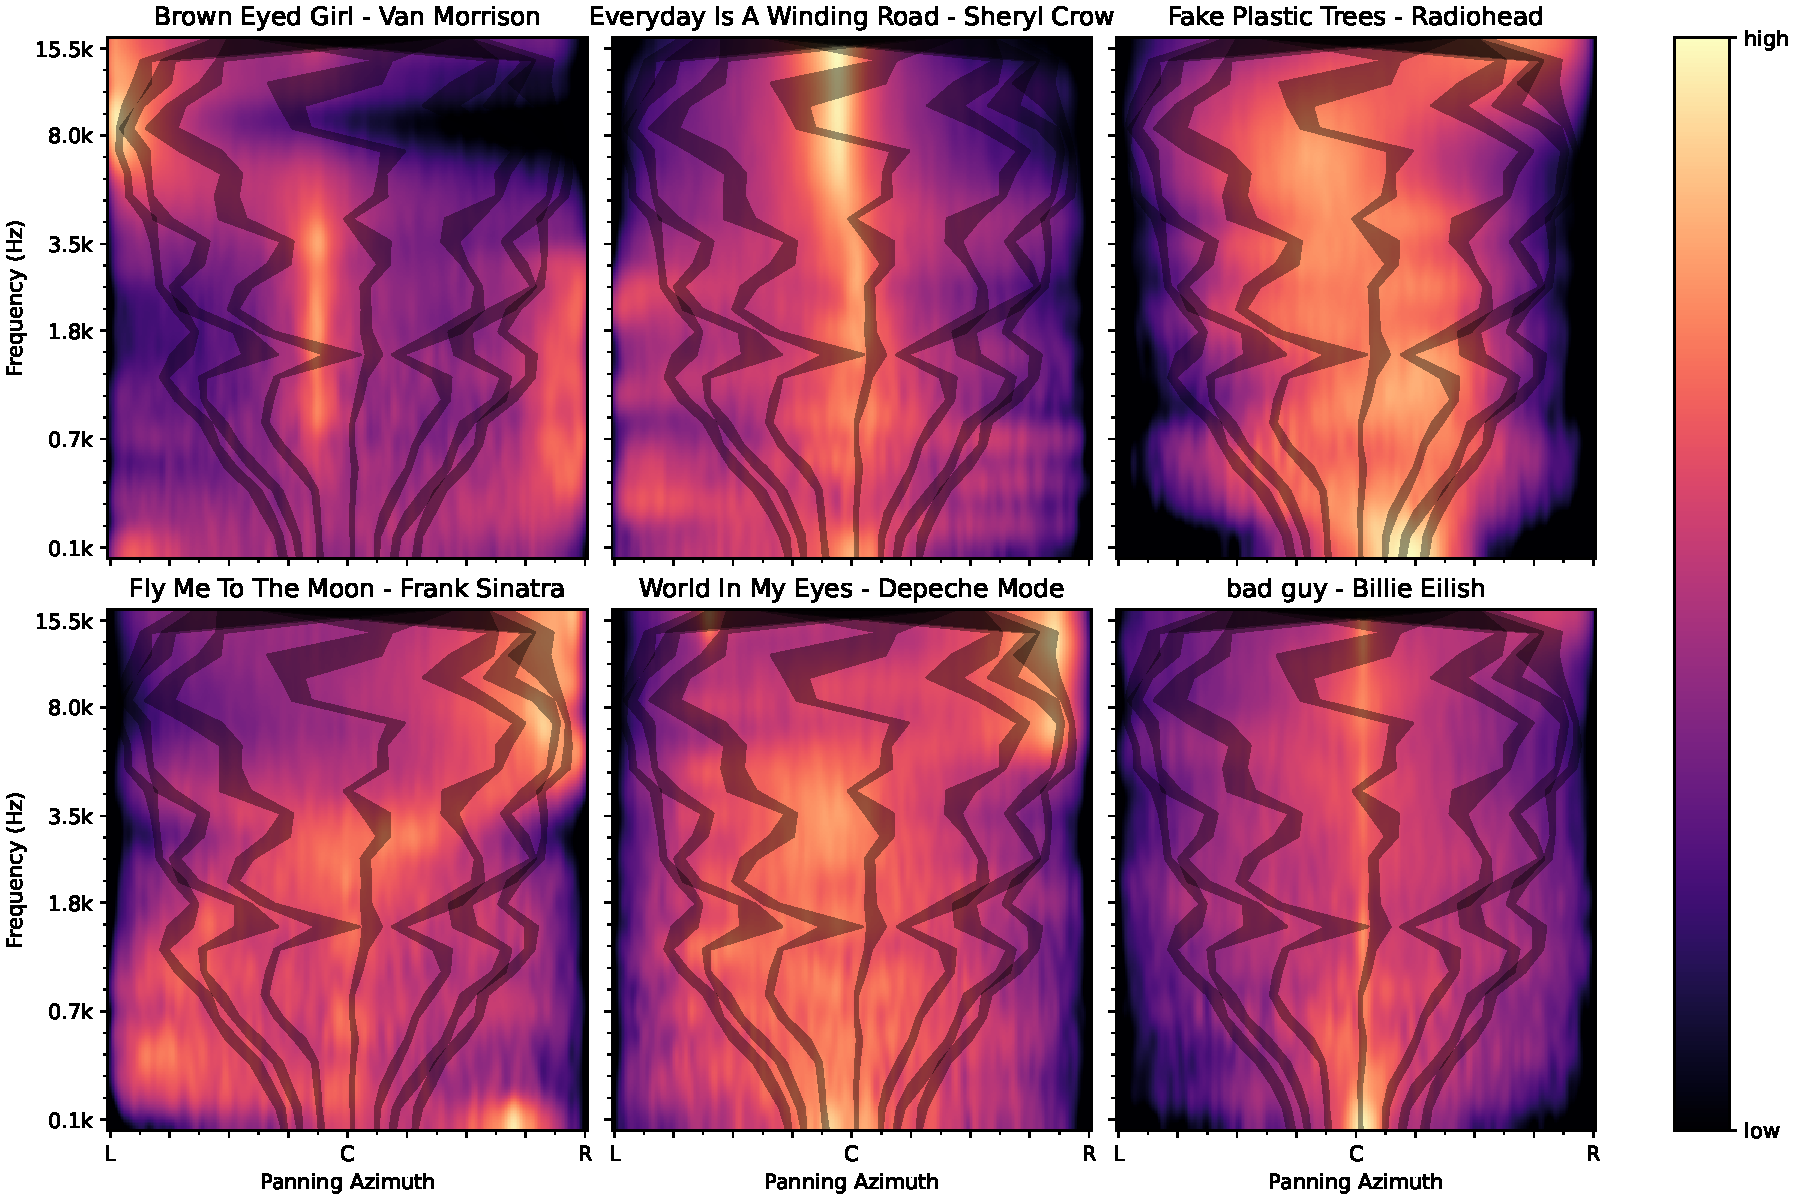
\includegraphics[width=0.8\columnwidth]{sips.pdf}
    \label{fig:sips}
    \caption{\acrlongpl{sip} of all tracks, with \glspl{sip} for all panned speech variants overlayed in grey. The colour scale is normalized for each track individually, with light and dark colours representing histogram peaks and troughs, respectively. Panning azimuth is a dimensionless value that ranges from left (L) to right (R), with centre (C) in the middle.}
\end{figure}

Comparing Fake Plastic Trees to all other tracks, it can be seen that the musical energy is spread quite evenly across the middle of the stereo field, and similarly across all frequency bands. In particular, all speech SIPs fall within frequency/azimuth regions where there is already a strong likelihood of musical energy. It is therefore theorized that the apparent randomness in participants' choices was caused by the lack of an obvious musical void in which to put panned speech. In an ideal case, it would be possible to correlate the randomness of the participants' scores with an objective measure derived from the SIPs. However, more music tracks would need to be analysed to gain enough data for a significant result. In \cite{bonett_sample_2000}, it is stated that a minimum of 25 items are required to obtain a reliable value of one of the standard correlation coefficients.

\subsection{Comparison of Ranked Azimuths}
\label{sec:comparison_of_ranked_azimuths}
To test for statistically significant differences between azimuths, a Kruskal-Wallis-H test is first conducted with the null hypothesis that all azimuths are ranked equally. With a confidence value of 95\% and seven azimuth classes, a critical value of $12.59$ is found in the $\chi^2$ distribution with six degrees of freedom~\cite{howell2013statistical}. The result of the test is an H-statistic of 18.0 with a p-value of 0.00636. Therefore, the null hypothesis is rejected and it can be concluded that at least one of the azimuths is ranked differently from the others. To determine which one, a Dunn's post-hoc test with Bonferroni correction is performed to compare pairwise p-values. The results of all pairs that included \enquote{Centre} are shown in Table~\ref{table:posthoc}. (All other pairs had p-values of 1 and are omitted from the table. There are two azimuths with a significant difference from \enquote{Centre} - \enquote{Left 45} and \enquote{Right 45}. Looking at the median scores of these two classes, it can be concluded that the extreme-panned speech were less highly rated than the more modest panned or centred speech. Interestingly, even though there are no other statistically significant differences, the \textit{confidence} of a difference from \enquote{Centre} is lower on the right side. We speculate that this might be due to the \enquote{right-ear advantage} -- a phenomenon in which a person is more easily able to interpret a voice presented to the right ear than the left \cite{tanaka_neurophysiological_2021}. More data would need to be collected to test this speculation.

Similar Kruskal-Wallis-H tests were performed with data for single tracks, but the null hypothesis could not be rejected for any of them.

\begin{table}[hb]
\centering
\begin{tabular}{lccccccc}
\toprule
 & Left 45 & Left 30 & Left 15 & Centre & Right 15 & Right 30 & Right 45 \\
\midrule
Median & 53.0 & 54.5 & 55.0 & 63.0 & 59.0 & 57.0 & 55.0 \\
P-value & \ovalbox{0.006} & 0.064 & 0.341 & 1.000 & 1.000 & 0.267 & \ovalbox{0.015} \\
\bottomrule
\end{tabular}
\caption{Medians and p-values for pairwise differences between the centre-panned voice and all other azimuths. Significant differences are circled.}
\label{table:posthoc}
\end{table}



\subsection{Analysis of Free-Text Responses}
To reiterate, the questions given to test participants with free-text responses were \enquote{Can you justify what influenced your ranking of spatialized voice in music?} and \enquote{Do you have any further feedback on the experiment?}. The participants answered both questions with similar information and therefore the responses were grouped. Subsequently, they were thematically analysed and classified by the authors. The themes mentioned are shown in Table~\ref{table:freetextthemes} alongside the number and percentage of participants who mentioned them.

The most prominent overarching theme was that difficulty in hearing the panned speech or its lack of clarity was the primary factor in the participants' ratings of pleasantness. Some participants provided more detailed feedback, specifying that the music was too loud or that the type of music affected their scores. Eight participants stated that they felt the voice was always clearer on either the left or the right, and seven stated that they always wanted the voice to be in the centre. Smaller sets of participants mentioned that clashes between any singing voice in the music and the speech led to lower ratings. They also noted that the pitch of the voice affected their ratings, either positively or negatively, depending on the music. A similarly small group mentioned that the spatial factors affected their scores.

\begin{table}[]
    \centering
    \begin{tabular}{lcc}
        \toprule
        Theme & Count & Percentage \\
        \midrule
        Clarity of voice / listening effort & 17 & 59\% \\
        Music too loud & 10 & 34\% \\
        Left/right preference & 8 & 28 \% \\
        Centre preference & 7 & 24\% \\
        Clash between singer and voice overlay & 5 & 17\% \\
        Speech pitch & 5 & 17\% \\
        Speech panning location / spatial factors & 4 & 14\% \\
        Music type / genre & 4 & 14\% \\
        \bottomrule
    \end{tabular}
    \caption{Counts of test participants who mentioned that specific factors affected their ratings.}
    \label{table:freetextthemes}
\end{table}

Based on these findings, it is suggested that further experiments stratify the music tracks into those with and without strong vocals, and include a more varied range of music genres among the tracks. Some comments also specifically mentioned that speech with more extreme panning was less pleasant, which is also reflected in the data (see Section~\ref{sec:comparison_of_ranked_azimuths}). It is therefore suggested that future tests use smaller increments of less extreme panning.


% \subsection{Graphs}

%\begin{figure}[t!]
%    \centering
%    \subfigure[Vocals only]{\includegraphics[trim=0.5cm 0cm 1.2cm 0cm, clip=true,width=0.43\columnwidth]{Spectrogram_VO_T1_summer.eps}}\vspace*{-0.3cm}
%   \subfigure[vocals on top of the music (Center)]{\includegraphics[trim=0.5cm 0cm 1.2cm 0cm, clip=true,width=0.43\columnwidth]{Spectrogram_C_T1_summer.eps}}
%   \label{fig:Spectogram_T1}\vspace*{-0.3cm}
%    \caption{Spectrograms of the left and right channels for Track 1, showing isolated vocals and vocals overlaid with music.}
%            \vspace{-0.3cm}
%\end{figure}
%

%\begin{figure}[t!]
%    \centering
%    \subfigure[Vocals only]{\includegraphics[trim=0.5cm 0cm 1.2cm 0cm, clip=true,width=0.43\columnwidth]{Spectrogram_VO_T2_summer.eps}}\vspace*{-0.3cm}
%   \subfigure[vocals on top of the music (Center)]{\includegraphics[trim=0.5cm 0cm 1.2cm 0cm, clip=true,width=0.43\columnwidth]{Spectrogram_C_T2_summer.eps}}
%   \label{fig:Spectogram_T2}\vspace*{-0.3cm}
%    \caption{Spectrograms of the left and right channels for Track 2, showing isolated vocals and vocals overlaid with music.}
%        \vspace{-0.3cm}
%\end{figure}
%

%\begin{figure}[t!]
%    \centering
%    \subfigure[Vocals only]{\includegraphics[trim=0.5cm 0cm 1.2cm 0cm, clip=true,width=0.43\columnwidth]{Spectrogram_VO_T3_summer.eps}}\vspace*{-0.3cm}
%   \subfigure[vocals on top of the music (Center)]{\includegraphics[trim=0.5cm 0cm 1.2cm 0cm, clip=true,width=0.43\columnwidth]{Spectrogram_C_T3_summer.eps}}
%   \label{fig:Spectogram_T3}\vspace*{-0.3cm}
%    \caption{Spectrograms of the left and right channels for Track 3, showing isolated vocals and vocals overlaid with music.}
%\end{figure}
%


%\begin{figure}[t!]
%    \centering
%    \subfigure[Vocals only]{\includegraphics[trim=0.5cm 0cm 1.2cm 0cm, clip=true,width=0.43\columnwidth]{Spectrogram_VO_T4_summer.eps}}\vspace*{-0.3cm}
%   \subfigure[vocals on top of the music (Center)]{\includegraphics[trim=0.5cm 0cm 1.2cm 0cm, clip=true,width=0.43\columnwidth]{Spectrogram_C_T4_summer.eps}}
%   \label{fig:Spectogram_T4}\vspace*{-0.3cm}
%    \caption{Spectrograms of the left and right channels for Track 4, showing isolated vocals and vocals overlaid with music.}
%            \vspace{-0.3cm}
%\end{figure}
%

%\begin{figure}[t!]
%    \centering
%    \subfigure[Vocals only]{\includegraphics[trim=0.5cm 0cm 1.2cm 0cm, clip=true,width=0.43\columnwidth]{Spectrogram_VO_T2_summer.eps}}\vspace*{-0.3cm}
%   \subfigure[vocals on top of the music (Center)]{\includegraphics[trim=0.5cm 0cm 1.2cm 0cm, clip=true,width=0.43\columnwidth]{Spectrogram_C_T5_summer.eps}}
%   \label{fig:Spectogram_T5}\vspace*{-0.3cm}
%    \caption{Spectrograms of the left and right channels for Track 5, showing isolated vocals and vocals overlaid with music.}
%        \vspace{-0.3cm}
%\end{figure}
%

%\begin{figure}[t!]
%    \centering
%    \subfigure[Vocals only]{\includegraphics[trim=0.5cm 0cm 1.2cm 0cm, clip=true,width=0.43\columnwidth]{Spectrogram_VO_T6_summer.eps}}\vspace*{-0.3cm}
%   \subfigure[vocals on top of the music (Center)]{\includegraphics[trim=0.5cm 0cm 1.2cm 0cm, clip=true,width=0.43\columnwidth]{Spectrogram_C_T6_summer.eps}}
%   \label{fig:Spectogram_T6}\vspace*{-0.3cm}
%    \caption{Spectrograms of the left and right channels for Track 6, showing isolated vocals and vocals overlaid with music.}
%\end{figure}
%

% \begin{figure}[t!]
%     %\vspace*{-0.5cm}
%     \centering
%     \subfigure[Track 1]{\includegraphics[trim=0.5cm 0cm 1.38cm 0.6cm, clip=true,width=0.33\columnwidth]{majed_img/Track1_rank_CI_v2.eps}}\vspace*{-0.05cm}
%    \subfigure[Track 2]{\includegraphics[trim=0.5cm 0cm 1.38cm 0.6cm, clip=true,width=0.33\columnwidth]{majed_img/Track2_rank_CI_v2.eps}}\vspace*{-0.05cm}
%    \subfigure[Track 3]{\includegraphics[trim=0.5cm 0cm 1.38cm 0.6cm, clip=true,width=0.33\columnwidth]{majed_img/Track3_rank_CI_v2.eps}}\\\vspace*{-0.3cm}
%    \subfigure[Track 4]{\includegraphics[trim=0.5cm 0cm 1.38cm 0.0cm, clip=true,width=0.33\columnwidth]{majed_img/Track4_rank_CI_v2.eps}}\vspace*{-0.05cm}
%    \subfigure[Track 5]{\includegraphics[trim=0.5cm 0cm 1.38cm 0.0cm, clip=true,width=0.33\columnwidth]{majed_img/Track5_rank_CI_v2.eps}}\vspace*{-0.05cm}
%    \subfigure[Track 6]{\includegraphics[trim=0.5cm 0cm 1.38cm 0.0cm, clip=true,width=0.33\columnwidth]{majed_img/Track6_rank_CI_v2.eps}}\vspace*{-0.05cm}\\\vspace*{-0.3cm}
%     \label{fig:MeanRank}
%     \caption{Mean ranked scores with different binaural panning angles for all the music tracks with 95\% confidence intervals.}
%     %\vspace{-0.4cm}
% \end{figure}
% %

% \begin{figure}[h]
%     %\vspace*{-0.5cm}
%     \centering
%     \subfigure[Track 1]{\includegraphics[trim=0.2cm 0cm 1.38cm 0.6cm, clip=true,width=0.33\columnwidth]{majed_img/Track1_freq_v2.eps}}\vspace*{-0.05cm}
%    \subfigure[Track 2]{\includegraphics[trim=0.2cm 0cm 1.38cm 0.6cm, clip=true,width=0.33\columnwidth]{majed_img/Track2_freq_v2.eps}}\vspace*{-0.05cm}
%    \subfigure[Track 3]{\includegraphics[trim=0.2cm 0cm 1.38cm 0.6cm, clip=true,width=0.33\columnwidth]{majed_img/Track3_freq_v2.eps}}\\\vspace*{-0.3cm}
%    \subfigure[Track 4]{\includegraphics[trim=0.2cm 0cm 1.38cm 0.0cm, clip=true,width=0.33\columnwidth]{majed_img/Track4_freq_v2.eps}}\vspace*{-0.05cm}
%    \subfigure[Track 5]{\includegraphics[trim=0.2cm 0cm 1.38cm 0.0cm, clip=true,width=0.33\columnwidth]{majed_img/Track5_freq_v2.eps}}\vspace*{-0.05cm}
%    \subfigure[Track 6]{\includegraphics[trim=0.2cm 0cm 1.38cm 0.0cm, clip=true,width=0.33\columnwidth]{majed_img/Track6_freq_v2.eps}}\\\vspace*{-0.3cm}
%     \label{fig:FreqRank1}
%     \caption{Frequency of first-ranked scores for all music tracks across different binaural panning angles. {\color{red} Is it possible to add some sort of confidence interval to these bars so we can prove that some tracks had a strong preference and others did not?} {\color{blue} These are just frequencies, so we may add probabilities on top of the bars?}}
% \end{figure}
% %

% \begin{figure}[h]
%     %\vspace*{-0.5cm}
%     \centering
%     \subfigure[Brown Eyed Girl]{\includegraphics[trim=0.2cm 0cm 1.38cm 0.6cm, clip=true,width=0.33\columnwidth]{majed_img/Track1_freq_RL_v2.eps}}\vspace*{-0.05cm}
%    \subfigure[Every Day Is A Winding Road]{\includegraphics[trim=0.2cm 0cm 1.38cm 0.6cm, clip=true,width=0.33\columnwidth]{majed_img/Track2_freq_RL_v2.eps}}\vspace*{-0.05cm}
%    \subfigure[Fake Plastic Trees]{\includegraphics[trim=0.2cm 0cm 1.38cm 0.6cm, clip=true,width=0.33\columnwidth]{majed_img/Track3_freq_RL_v2.eps}}\\\vspace*{-0.3cm}
%    \subfigure[Fly Me To The Moon]{\includegraphics[trim=0.2cm 0cm 1.38cm 0.0cm, clip=true,width=0.33\columnwidth]{majed_img/Track4_freq_RL_v2.eps}}\vspace*{-0.05cm}
%    \subfigure[World In My Eyes]{\includegraphics[trim=0.2cm 0cm 1.38cm 0.0cm, clip=true,width=0.33\columnwidth]{majed_img/Track5_freq_RL_v2.eps}}\vspace*{-0.05cm}
%    \subfigure[Bad Guy]{\includegraphics[trim=0.2cm 0cm 1.38cm 0.0cm, clip=true,width=0.33\columnwidth]{majed_img/Track6_freq_RL_v2.eps}}\\\vspace*{-0.3cm}
%     \label{fig:FreqRank1}
%     \caption{Frequency of first-ranked scores for all music tracks, based on the sum of the right and left binaural panning angles.}
% \end{figure}
% %

% \begin{figure}[t!]
%     %\vspace*{-0.5cm}
%     \centering
%     \subfigure[Brown Eyed Girl]{\includegraphics[trim=0.1cm 0cm 0cm 0.6cm, clip=true,width=0.33\columnwidth]{majed_img/Freq_Azimuth_T1.eps}}\vspace*{-0.05cm}
%    \subfigure[Every Day Is A Winding Road]{\includegraphics[trim=0.1cm 0cm 0cm 0.6cm, clip=true,width=0.33\columnwidth]{majed_img/Freq_Azimuth_T2.eps}}\vspace*{-0.05cm}
%    \subfigure[Fake Plastic Trees]{\includegraphics[trim=0.1cm 0cm 0cm 0.6cm, clip=true,width=0.33\columnwidth]{majed_img/Freq_Azimuth_T3.eps}}\\\vspace*{-0.3cm}
%    \subfigure[Fly Me To The Moon]{\includegraphics[trim=0.1cm 0cm 0cm 0.0cm, clip=true,width=0.33\columnwidth]{majed_img/Freq_Azimuth_T4.eps}}\vspace*{-0.05cm}
%    \subfigure[World In My Eyes]{\includegraphics[trim=0.1cm 0cm 0cm 0.0cm, clip=true,width=0.33\columnwidth]{majed_img/Freq_Azimuth_T5.eps}}\vspace*{-0.05cm}
%    \subfigure[Bad Guy]{\includegraphics[trim=0.1cm 0cm 0cm 0.0cm, clip=true,width=0.33\columnwidth]{majed_img/Freq_Azimuth_T6.eps}}\vspace*{-0.05cm}\\\vspace*{-0.3cm}
%     \label{fig:MeanRank}
%     \caption{Frequency-Azimuth spectrogram for all the music tracks. {\color{red}Can we display the frequency axis in logarithmic scale? Is the X-axis really binaural panning angle? In our previous work it is referred to just as an azimuth which does not necessarily have a physical property linked to it. We should also specify the algorithm that generates these plots.}}
%     %\vspace{-0.4cm}
% \end{figure}
% %


% \begin{figure}[h]
%     %\vspace*{-0.5cm}
%     \centering
%     \subfigure[Brown Eyed Girl]{\includegraphics[trim=0.2cm 0cm 1.38cm 0.6cm, clip=true,width=0.33\columnwidth]{majed_img/combo_T1.eps}}\vspace*{-0.05cm}
%    \subfigure[Every Day Is A Winding Road]{\includegraphics[trim=0.2cm 0cm 1.38cm 0.6cm, clip=true,width=0.33\columnwidth]{majed_img/combo_T2.eps}}\vspace*{-0.05cm}
%    \subfigure[Fake Plastic Trees]{\includegraphics[trim=0.2cm 0cm 1.38cm 0.6cm, clip=true,width=0.33\columnwidth]{majed_img/combo_T3.eps}}\\\vspace*{-0.3cm}
%    \subfigure[Fly Me To The Moon]{\includegraphics[trim=0.2cm 0cm 1.38cm 0.0cm, clip=true,width=0.33\columnwidth]{majed_img/combo_T4.eps}}\vspace*{-0.05cm}
%    \subfigure[World In My Eyes]{\includegraphics[trim=0.2cm 0cm 1.38cm 0.0cm, clip=true,width=0.33\columnwidth]{majed_img/combo_T5.eps}}\vspace*{-0.05cm}
%    \subfigure[Bad Guy]{\includegraphics[trim=0.2cm 0cm 1.38cm 0.0cm, clip=true,width=0.33\columnwidth]{majed_img/combo_T6.eps}}\\\vspace*{-0.3cm}
%     \label{fig:FreqRank1}
%     \caption{Frequency of first-ranked scores for all music tracks, based on the sum of the right and left binaural panning angles.}
% \end{figure}
% %

% \subsection{Experience levels}\label{ResultsAnalysis}

% \begin{figure}[h]
%     %\vspace*{-0.5cm}
%     \centering
%     \subfigure[Brown Eyed Girl]{\includegraphics[trim=0.1cm 0.2cm 0cm 1cm, clip=true,width=0.22\columnwidth]{majed_img/Freq_Azimuth_T1.eps}}\vspace*{-0.05cm}
%     \subfigure[Experience listener]{\includegraphics[width=0.22\columnwidth]{majed_img/Track1_freq_RL_v2_yes.eps}}\vspace*{-0.05cm}
%    \subfigure[Do not know]{\includegraphics[width=0.22\columnwidth]{majed_img/Track1_freq_RL_v2_dk.eps}}\vspace*{-0.05cm}
%    \subfigure[Non experience listener]{\includegraphics[width=0.22\columnwidth]{majed_img/Track1_freq_RL_v2_no.eps}}\\\vspace*{-0.3cm}
%     \subfigure[Every Day Is A Winding Road]{\includegraphics[trim=0.1cm 0cm 0cm 0.6cm, clip=true,width=0.22\columnwidth]{majed_img/Freq_Azimuth_T2.eps}}\vspace*{-0.05cm}
%    \subfigure[Experience listener]{\includegraphics[width=0.22\columnwidth]{majed_img/Track2_freq_RL_v2_yes.eps}}\vspace*{-0.05cm}
%    \subfigure[Do not know]{\includegraphics[width=0.22\columnwidth]{majed_img/Track2_freq_RL_v2_dk.eps}}\vspace*{-0.05cm}
%    \subfigure[Non experience listener]{\includegraphics[width=0.22\columnwidth]{majed_img/Track2_freq_RL_v2_no.eps}}\\\vspace*{-0.3cm}
%     \subfigure[Fake Plastic Trees]{\includegraphics[trim=0.1cm 0cm 0cm 0.6cm, clip=true,width=0.22\columnwidth]{majed_img/Freq_Azimuth_T3.eps}}\vspace*{-0.05cm}
%    \subfigure[Experience listener]{\includegraphics[width=0.22\columnwidth]{majed_img/Track3_freq_RL_v2_yes.eps}}\vspace*{-0.05cm}
%    \subfigure[Do not know]{\includegraphics[width=0.22\columnwidth]{majed_img/Track3_freq_RL_v2_dk.eps}}\vspace*{-0.05cm}
%    \subfigure[Non experience listener]{\includegraphics[width=0.22\columnwidth]{majed_img/Track3_freq_RL_v2_no.eps}}\\\vspace*{-0.3cm}
%     \subfigure[Fly Me To The Moon]{\includegraphics[trim=0.1cm 0cm 0cm 0.6cm, clip=true,width=0.22\columnwidth]{majed_img/Freq_Azimuth_T4.eps}}\vspace*{-0.05cm}
%     \subfigure[Experience listener]{\includegraphics[width=0.22\columnwidth]{majed_img/Track4_freq_RL_v2_yes.eps}}\vspace*{-0.05cm}
%    \subfigure[Do not know]{\includegraphics[width=0.22\columnwidth]{majed_img/Track4_freq_RL_v2_dk.eps}}\vspace*{-0.05cm}
%    \subfigure[Non experience listener]{\includegraphics[width=0.22\columnwidth]{majed_img/Track4_freq_RL_v2_no.eps}}\\\vspace*{-0.3cm}
%     \subfigure[World In My Eyes]{\includegraphics[trim=0.1cm 0cm 0cm 0.6cm, clip=true,width=0.22\columnwidth]{majed_img/Freq_Azimuth_T5.eps}}\vspace*{-0.05cm}
%     \subfigure[Experience listener]{\includegraphics[width=0.22\columnwidth]{majed_img/Track5_freq_RL_v2_yes.eps}}\vspace*{-0.05cm}
%    \subfigure[Do not know]{\includegraphics[width=0.22\columnwidth]{majed_img/Track5_freq_RL_v2_dk.eps}}\vspace*{-0.05cm}
%    \subfigure[Non experience listener]{\includegraphics[width=0.22\columnwidth]{majed_img/Track5_freq_RL_v2_no.eps}}\\\vspace*{-0.3cm}
%     \subfigure[Bad Guy]{\includegraphics[trim=0.1cm 0cm 0cm 0.6cm, clip=true,width=0.22\columnwidth]{majed_img/Freq_Azimuth_T6.eps}}\vspace*{-0.05cm}
%     \subfigure[Experience listener]{\includegraphics[width=0.22\columnwidth]{majed_img/Track6_freq_RL_v2_yes.eps}}\vspace*{-0.05cm}
%    \subfigure[Do not know]{\includegraphics[width=0.22\columnwidth]{majed_img/Track6_freq_RL_v2_dk.eps}}\vspace*{-0.05cm}
%    \subfigure[Non experience listener]{\includegraphics[width=0.22\columnwidth]{majed_img/Track6_freq_RL_v2_no.eps}}\\\vspace*{-0.3cm}


%     \label{fig:RL_exp}
%     \caption{Experience levels. Figures to be improved later.}
% \end{figure}
%

% \clearpage

%Majed/All:

% Ratings of voice+music
% {\color{blue} Based on the recorded data, we can see the MUSHRA rating scores of voice+music for the different setups, including the angles \{45L, 30L, 15L, 0, 15R, 30R, 45R\} we average over the participants. We can do (1) for mean MUSHRA Scores versus each voice+ each music  (2) for average mean MUSHRA Scores versus all voice+ all music  (3) split for male and female for all voice+ all music} 

% Preference angles data
% {\color{blue} do you have more info? I believe this will relate to the first point about ratings of voice and music where the angles will be revealed. A statistical test can be done to see if there is a difference between the angles}

% Preference male/female data
% {\color{blue} Will also be reviled one we have the ratings of the voices+music when we split by gender and averaging all) can be done with (1) average all the scores for the music+voice (2) foe each music+voice}

% Duration spent on each song, did they spend longer on certain song+voice combinations?
% {\color{blue} here we have a bad news. I found that the time is recorded when you just click on the next. So, the starting time of the experiment is not counted. In this case we can not know the duration of the first music+voice}

% Justifications of what influenced the ranking of spatialized voice in music
% {\color{blue} This will be shown when we have the test results from the questionnaire}

% Preference for female or male voice in music - based on gender
% {\color{blue} This will be shown when we have the test results from the questionnaire}

%Relationships between the volume of voice and music
%{\color{blue} This will be shown when we have the test results from the questionnaire}

% Other feedback
% {\color{blue} nice points, we can split further based on participants' experience levels etc.. }

%{\color{blue}
%\begin{itemize}
%    \item Do you think we need to calculate the SNR for each music+song and see the correlation with the score?? Since I am new to this field, do you think changing the angle will change the SNR?? or it is the same anyway which I do not think so?
%    \item if that works, we can see the score for each music+sound and we can split by gender/ right and left angles etc...
%    \item  What do you think if we got the difference score between the center ant the rest of angles for instance \begin{equation}
%    \text{difference\_in\_score} = \left| \text{Score}_{0} - \text{socre}_{15R} \right|
%    \label{eq:score_difference}
%\end{equation}
%\item I am not sure it is just came to my mind and wrote it
%\item if reference is always 100, do we have a metric like DMOS? taking the difference from the reference ? is it important as which in the videos and we have the reference is not hidden I see it is important but let me check the recommendations. 
%\end{itemize}}

%\begin{table}[h]
%    \centering
%    \caption{Signal to noise ratio for Bad guy + Billie Eilish for the different binaural panning. }
%    \begin{tabular}{c|c|c|c|c|c|c|c|c}
%        \hline
%           &Ref.    &45L    &30L    &15L    &0    &15R    &30R   &45R\\ \hline
%     Left (dB)   &4.62    &\textbf{5.51}    &5.38    &5.14    &4.83    &4.66    &4.57    &4.56\\ \hline
%     Right (dB)  &4.18    &3.97    &4.01    &4.13    &4.41    &4.69    &4.91    &\textbf{5.00}\\ \hline
%     Average(dB) &4.40    &4.74    &4.69    &4.64    &4.62    &4.67    &4.74    & \textbf{4.78} \\ \hline
%    \end{tabular}
    
%    \label{SNR}
%\end{table}

%Table \ref{SNR} Just a test. I could have bugs in the 10-minute code. We will not have this in the paper, but I just was wondering if the SNR is the same or not. I am not sure about my calculations- Let me know Richard if you have comments on this. I would interpret this as 45R has the highest signal-to-noise ratio, which may be used for prediction or such.. Once we have the scores we can see the correlation. But I need to make sure that I have the correct results :)
% \begin{figure}
%     %\vspace*{-0.5cm}
%     \centering
%     \subfigure[Ranked scores]{\includegraphics[trim=0.5cm 0cm 1.38cm 0cm, clip=true,width=0.33\columnwidth]{majed_img/average_mean_rankedScore.eps}}\vspace*{-0.05cm}
%     \subfigure[Frequency of rank 1 scores]{\includegraphics[trim=0.5cm 0cm 1.38cm 0cm, clip=true,width=0.33\columnwidth]{majed_img/combo_split_all.eps}}\subfigure[Frequency of rank 1 scores]{\includegraphics[trim=0.5cm 0cm 1.38cm 0cm, clip=true,width=0.33\columnwidth]{majed_img/combo_all.eps}}\\
%     \label{fig:QP_AverageMOS}
%     \caption{Average All tracks.}
%     %\vspace{-0.4cm}
% \end{figure}

\subsection{Discussion}\label{Discussion}
%All:
A constant source of uncertainty during data analysis was the relatively small number of both tracks and participants. In particular, only six tracks were used to limit the duration of each test session. In reality, it was not enough to draw statistical conclusions about differences between tracks. 

Furthermore, several of the statistical tests used (e.g., the binomial test in Section~\ref{sec:noncentrepref}) are based on the assumption that all data are independent. It could be argued that the data collected are not strictly independent since each participant scored multiple tracks. This was a practical compromise made to gather enough data for any analysis. It is a known problem that subjective tests of this variety are slow and costly, and recent efforts in crowdsourcing \gls{mushra} tests have proven fruitful \cite{lechler_crowdsourcing_2025} (although this work focused on assessing solo speech signals rather than music).

\section{Conclusions and Future Work}
\label{Conclusions}
A perceptual evaluation was performed to determine the pleasantness of music mixed with voice that has been binaurally panned to various angles by convolving the signal with an \gls{hrir}. Participants were presented with a \gls{mushra}-like test in which they moved sliders to give their opinions of the different panning azimuths. The raw scores were transformed into ranks on a per-person-per-track basis.

Binomial tests on the top-ranked azimuth revealed that the non-centre positions were preferred over the centre, although with the limited data collected in this experiment, it was not possible to analyse further. More data, particularly a higher number of tracks, is necessary to determine the cause of the preference.

Kruskal-Wallis tests revealed that the outermost azimuths were consistently ranked lower than the moderately panned and centre azimuths. There was also the implication that the voice panned to the right was ranked higher than that on the left, but as stated above, more data would be required for confirmation.

The free-text explanations given by the participants showed that \enquote{listening effort} or \enquote{voice clarity} were the factors that influenced the pleasantness of the audio for the highest number of people. Alongside this were indications that other factors relating to listeners' personal preference and the interplay of speech and music should be investigated in future experiments.

Based on these findings, we suggest that further experiments be performed in which 
\begin{enumerate*}
    \item more tracks and more test participants are used,
    \item the musical excerpts chosen are controlled so that they have either strong vocals or a lack thereof throughout,
    \item the vocal overlays are panned more towards the centre and in finer increments.
\end{enumerate*}

% \section{Future Work}
% \label{FutureWork}
%All:



\begin{acks}
This research was funded in part by the Knowledge Foundation, Sweden, through the \gls{hints} Profile Project (contract 20220068). The authors thank all the volunteers who participated in the experiment.
\end{acks}

%%
%% The next two lines define the bibliography style to be used, and
%% the bibliography file.
\bibliographystyle{ACM-Reference-Format}
\bibliography{bibliography}

%\clearpage

%%
%% If your work has an appendix, this is the place to put it.
%\appendix

%\section{Appendix ??}\label{??}

%\subsection{General information (tb be removed later)}
%My agenda:
%\begin{itemize}
%    \item \sout{For perceptual ranked scores, I will flip the y-axis and start with Rank 7 to Rank 1 so the figure will make more sense (Done).}
%    \item \sout{I will produce the histograms for all the ranks, starting from 1 (Done) to 7, in the appendix. It is time for other ranks (working on). About adding the figures in the appendix }
 %   \item \sout{From the frequencies, I will aggregate all binaural panning angles compared to zero panning angles. (Done) But probably I will do for all the ranks (under progress). }
 %   \item \sout{Expecting to finish the above two points by tomorrow, 14th of August.}
 %   \item \sout{Working on Spectrogram figures to motivate the findings (Done) }


    
%    \item \sout{Split the above results into three categories related to music experience: Yes, No, I do not know (luckily, we have almost equal experience groups).}
%    \item I will then move to see what we have in the paper, so I can add and write starting from the results
    
%\end{itemize}



%%%%%%%%%%%%%%%%%%%%%%%%%%%%%%%%%%%%%%%%%%%%%%%%%%%%%%%%%%%%%%%%%%
%%%%%%%%%%%%%%%%%%%%% Frequency distribution of rank scores %%%%%%
%%%%%%%%%%%%%%%%%%%%%%%%%%%%%%%%%%%%%%%%%%%%%%%%%%%%%%%%%%%%%%%%%%

\begin{comment}
    
\clearpage

\subsection{Frequency Distribution of Rank Scores for Track 1}

\begin{figure}[h]
    %\vspace*{-0.5cm}
    \centering
    \subfigure[Second-Ranked]{\includegraphics[width=0.3\columnwidth]{majed_img/Track1_freq_v2_2.eps}}\vspace*{-0.05cm}
   \subfigure[Third-Ranked]{\includegraphics[width=0.3\columnwidth]{majed_img/Track1_freq_v2_3.eps}}\vspace*{-0.05cm}
   \subfigure[Fourth-Ranked]{\includegraphics[width=0.3\columnwidth]{majed_img/Track1_freq_v2_4.eps}}\\\vspace*{-0.3cm}
   \subfigure[Fifth-Ranked]{\includegraphics[width=0.3\columnwidth]{majed_img/Track1_freq_v2_5.eps}}\vspace*{-0.05cm}
   \subfigure[Sixth-Ranked]{\includegraphics[width=0.3\columnwidth]{majed_img/Track1_freq_v2_6.eps}}\vspace*{-0.05cm}
   \subfigure[Seventh-Ranked]{\includegraphics[width=0.3\columnwidth]{majed_img/Track1_freq_v2_7.eps}}\\\vspace*{-0.3cm}
    \label{fig:FreqRank_track1}
    \caption{Frequency distribution of rank scores for Track 1 at varying binaural panning angles.}
\end{figure}
%

\begin{figure}[h]
    %\vspace*{-0.5cm}
    \centering
    \subfigure[Second-Ranked]{\includegraphics[width=0.3\columnwidth]{majed_img/Track1_freq_RL_v2_2.eps}}\vspace*{-0.05cm}
   \subfigure[Third-Ranked]{\includegraphics[width=0.3\columnwidth]{majed_img/Track1_freq_RL_v2_3.eps}}\vspace*{-0.05cm}
   \subfigure[Fourth-Ranked]{\includegraphics[width=0.3\columnwidth]{majed_img/Track1_freq_RL_v2_4.eps}}\\\vspace*{-0.3cm}
   \subfigure[Fifth-Ranked]{\includegraphics[width=0.3\columnwidth]{majed_img/Track1_freq_RL_v2_5.eps}}\vspace*{-0.05cm}
   \subfigure[Sixth-Ranked]{\includegraphics[width=0.3\columnwidth]{majed_img/Track1_freq_RL_v2_6.eps}}\vspace*{-0.05cm}
   \subfigure[Seventh-Ranked]{\includegraphics[width=0.3\columnwidth]{majed_img/Track1_freq_RL_v2_7.eps}}\\\vspace*{-0.3cm}
    \label{fig:FreqRank_track1}
    \caption{Frequency distribution of rank scores for Track 1 based on the sum of the right and left binaural panning angles.}
\end{figure}
%

\subsection{Frequency Distribution of Rank Scores for Track 2}

\begin{figure}[h]
    %\vspace*{-0.5cm}
    \centering
    \subfigure[Second-Ranked]{\includegraphics[width=0.3\columnwidth]{majed_img/Track2_freq_v2_2.eps}}\vspace*{-0.05cm}
   \subfigure[Third-Ranked]{\includegraphics[width=0.3\columnwidth]{majed_img/Track2_freq_v2_3.eps}}\vspace*{-0.05cm}
   \subfigure[Fourth-Ranked]{\includegraphics[width=0.3\columnwidth]{majed_img/Track2_freq_v2_4.eps}}\\\vspace*{-0.3cm}
   \subfigure[Fifth-Ranked]{\includegraphics[width=0.3\columnwidth]{majed_img/Track2_freq_v2_5.eps}}\vspace*{-0.05cm}
   \subfigure[Sixth-Ranked]{\includegraphics[width=0.3\columnwidth]{majed_img/Track2_freq_v2_6.eps}}\vspace*{-0.05cm}
   \subfigure[Seventh-Ranked]{\includegraphics[width=0.3\columnwidth]{majed_img/Track2_freq_v2_7.eps}}\\\vspace*{-0.3cm}
    \label{fig:FreqRank_track2}
    \caption{Frequency distribution of rank scores for Track 2 at varying binaural panning angles.}
\end{figure}
%

\begin{figure}[h]
    %\vspace*{-0.5cm}
    \centering
    \subfigure[Second-Ranked]{\includegraphics[width=0.3\columnwidth]{majed_img/Track2_freq_RL_v2_2.eps}}\vspace*{-0.05cm}
   \subfigure[Third-Ranked]{\includegraphics[width=0.3\columnwidth]{majed_img/Track2_freq_RL_v2_3.eps}}\vspace*{-0.05cm}
   \subfigure[Fourth-Ranked]{\includegraphics[width=0.3\columnwidth]{majed_img/Track2_freq_RL_v2_4.eps}}\\\vspace*{-0.3cm}
   \subfigure[Fifth-Ranked]{\includegraphics[width=0.3\columnwidth]{majed_img/Track2_freq_RL_v2_5.eps}}\vspace*{-0.05cm}
   \subfigure[Sixth-Ranked]{\includegraphics[width=0.3\columnwidth]{majed_img/Track2_freq_RL_v2_6.eps}}\vspace*{-0.05cm}
   \subfigure[Seventh-Ranked]{\includegraphics[width=0.3\columnwidth]{majed_img/Track2_freq_RL_v2_7.eps}}\\\vspace*{-0.3cm}
    \label{fig:FreqRank_track2}
    \caption{Frequency distribution of rank scores for Track 2 based on the sum of the right and left binaural panning angles.}
\end{figure}
%

\subsection{Frequency Distribution of Rank Scores for Track 3}

\begin{figure}[h]
    %\vspace*{-0.5cm}
    \centering
    \subfigure[Second-Ranked]{\includegraphics[width=0.3\columnwidth]{majed_img/Track3_freq_v2_2.eps}}\vspace*{-0.05cm}
   \subfigure[Third-Ranked]{\includegraphics[width=0.3\columnwidth]{majed_img/Track3_freq_v2_3.eps}}\vspace*{-0.05cm}
   \subfigure[Fourth-Ranked]{\includegraphics[width=0.3\columnwidth]{majed_img/Track3_freq_v2_4.eps}}\\\vspace*{-0.3cm}
   \subfigure[Fifth-Ranked]{\includegraphics[width=0.3\columnwidth]{majed_img/Track3_freq_v2_5.eps}}\vspace*{-0.05cm}
   \subfigure[Sixth-Ranked]{\includegraphics[width=0.3\columnwidth]{majed_img/Track3_freq_v2_6.eps}}\vspace*{-0.05cm}
   \subfigure[Seventh-Ranked]{\includegraphics[width=0.3\columnwidth]{majed_img/Track3_freq_v2_7.eps}}\\\vspace*{-0.3cm}
    \label{fig:FreqRank_track3}
    \caption{Frequency distribution of rank scores for Track 3 at varying binaural panning angles.}
\end{figure}
%

\begin{figure}[h]
    %\vspace*{-0.5cm}
    \centering
    \subfigure[Second-Ranked]{\includegraphics[width=0.3\columnwidth]{majed_img/Track3_freq_RL_v2_2.eps}}\vspace*{-0.05cm}
   \subfigure[Third-Ranked]{\includegraphics[width=0.3\columnwidth]{majed_img/Track3_freq_RL_v2_3.eps}}\vspace*{-0.05cm}
   \subfigure[Fourth-Ranked]{\includegraphics[width=0.3\columnwidth]{majed_img/Track3_freq_RL_v2_4.eps}}\\\vspace*{-0.3cm}
   \subfigure[Fifth-Ranked]{\includegraphics[width=0.3\columnwidth]{majed_img/Track3_freq_RL_v2_5.eps}}\vspace*{-0.05cm}
   \subfigure[Sixth-Ranked]{\includegraphics[width=0.3\columnwidth]{majed_img/Track3_freq_RL_v2_6.eps}}\vspace*{-0.05cm}
   \subfigure[Seventh-Ranked]{\includegraphics[width=0.3\columnwidth]{majed_img/Track3_freq_RL_v2_7.eps}}\\\vspace*{-0.3cm}
    \label{fig:FreqRank_track3}
    \caption{Frequency distribution of rank scores for Track 3 based on the sum of the right and left binaural panning angles.}
\end{figure}
%

\subsection{Frequency Distribution of Rank Scores for Track 4}

\begin{figure}[h]
    %\vspace*{-0.5cm}
    \centering
    \subfigure[Second-Ranked]{\includegraphics[width=0.3\columnwidth]{majed_img/Track4_freq_v2_2.eps}}\vspace*{-0.05cm}
   \subfigure[Third-Ranked]{\includegraphics[width=0.3\columnwidth]{majed_img/Track4_freq_v2_3.eps}}\vspace*{-0.05cm}
   \subfigure[Fourth-Ranked]{\includegraphics[width=0.3\columnwidth]{majed_img/Track4_freq_v2_4.eps}}\\\vspace*{-0.3cm}
   \subfigure[Fifth-Ranked]{\includegraphics[width=0.3\columnwidth]{majed_img/Track4_freq_v2_5.eps}}\vspace*{-0.05cm}
   \subfigure[Sixth-Ranked]{\includegraphics[width=0.3\columnwidth]{majed_img/Track4_freq_v2_6.eps}}\vspace*{-0.05cm}
   \subfigure[Seventh-Ranked]{\includegraphics[width=0.3\columnwidth]{majed_img/Track4_freq_v2_7.eps}}\\\vspace*{-0.3cm}
    \label{fig:FreqRank_track4}
    \caption{Frequency distribution of rank scores for Track 4 at varying binaural panning angles.}
\end{figure}
%

\begin{figure}[h]
    %\vspace*{-0.5cm}
    \centering
    \subfigure[Second-Ranked]{\includegraphics[width=0.3\columnwidth]{majed_img/Track4_freq_RL_v2_2.eps}}\vspace*{-0.05cm}
   \subfigure[Third-Ranked]{\includegraphics[width=0.3\columnwidth]{majed_img/Track4_freq_RL_v2_3.eps}}\vspace*{-0.05cm}
   \subfigure[Fourth-Ranked]{\includegraphics[width=0.3\columnwidth]{majed_img/Track4_freq_RL_v2_4.eps}}\\\vspace*{-0.3cm}
   \subfigure[Fifth-Ranked]{\includegraphics[width=0.3\columnwidth]{majed_img/Track4_freq_RL_v2_5.eps}}\vspace*{-0.05cm}
   \subfigure[Sixth-Ranked]{\includegraphics[width=0.3\columnwidth]{majed_img/Track4_freq_RL_v2_6.eps}}\vspace*{-0.05cm}
   \subfigure[Seventh-Ranked]{\includegraphics[width=0.3\columnwidth]{majed_img/Track4_freq_RL_v2_7.eps}}\\\vspace*{-0.3cm}
    \label{fig:FreqRank_track4}
    \caption{Frequency distribution of rank scores for Track 4 based on the sum of the right and left binaural panning angles.}
\end{figure}
%


\subsection{Frequency Distribution of Rank Scores for Track 5}

\begin{figure}[h]
    %\vspace*{-0.5cm}
    \centering
    \subfigure[Second-Ranked]{\includegraphics[width=0.3\columnwidth]{majed_img/Track5_freq_v2_2.eps}}\vspace*{-0.05cm}
   \subfigure[Third-Ranked]{\includegraphics[width=0.3\columnwidth]{majed_img/Track5_freq_v2_3.eps}}\vspace*{-0.05cm}
   \subfigure[Fourth-Ranked]{\includegraphics[width=0.3\columnwidth]{majed_img/Track5_freq_v2_4.eps}}\\\vspace*{-0.3cm}
   \subfigure[Fifth-Ranked]{\includegraphics[width=0.3\columnwidth]{majed_img/Track5_freq_v2_5.eps}}\vspace*{-0.05cm}
   \subfigure[Sixth-Ranked]{\includegraphics[width=0.3\columnwidth]{majed_img/Track5_freq_v2_6.eps}}\vspace*{-0.05cm}
   \subfigure[Seventh-Ranked]{\includegraphics[width=0.3\columnwidth]{majed_img/Track5_freq_v2_7.eps}}\\\vspace*{-0.3cm}
    \label{fig:FreqRank_track5}
    \caption{Frequency distribution of rank scores for Track 5 at varying binaural panning angles.}
\end{figure}
%

\begin{figure}[h]
    %\vspace*{-0.5cm}
    \centering
    \subfigure[Second-Ranked]{\includegraphics[width=0.3\columnwidth]{majed_img/Track5_freq_RL_v2_2.eps}}\vspace*{-0.05cm}
   \subfigure[Third-Ranked]{\includegraphics[width=0.3\columnwidth]{majed_img/Track5_freq_RL_v2_3.eps}}\vspace*{-0.05cm}
   \subfigure[Fourth-Ranked]{\includegraphics[width=0.3\columnwidth]{majed_img/Track5_freq_RL_v2_4.eps}}\\\vspace*{-0.3cm}
   \subfigure[Fifth-Ranked]{\includegraphics[width=0.3\columnwidth]{majed_img/Track5_freq_RL_v2_5.eps}}\vspace*{-0.05cm}
   \subfigure[Sixth-Ranked]{\includegraphics[width=0.3\columnwidth]{majed_img/Track5_freq_RL_v2_6.eps}}\vspace*{-0.05cm}
   \subfigure[Seventh-Ranked]{\includegraphics[width=0.3\columnwidth]{majed_img/Track5_freq_RL_v2_7.eps}}\\\vspace*{-0.3cm}
    \label{fig:FreqRank_track5}
    \caption{Frequency distribution of rank scores for Track 5 based on the sum of the right and left binaural panning angles.}
\end{figure}
%


\subsection{Frequency Distribution of Rank Scores for Track 6}

\begin{figure}[h]
    %\vspace*{-0.5cm}
    \centering
    \subfigure[Second-Ranked]{\includegraphics[width=0.3\columnwidth]{majed_img/Track6_freq_v2_2.eps}}\vspace*{-0.05cm}
   \subfigure[Third-Ranked]{\includegraphics[width=0.3\columnwidth]{majed_img/Track6_freq_v2_3.eps}}\vspace*{-0.05cm}
   \subfigure[Fourth-Ranked]{\includegraphics[width=0.3\columnwidth]{majed_img/Track6_freq_v2_4.eps}}\\\vspace*{-0.3cm}
   \subfigure[Fifth-Ranked]{\includegraphics[width=0.3\columnwidth]{majed_img/Track6_freq_v2_5.eps}}\vspace*{-0.05cm}
   \subfigure[Sixth-Ranked]{\includegraphics[width=0.3\columnwidth]{majed_img/Track6_freq_v2_6.eps}}\vspace*{-0.05cm}
   \subfigure[Seventh-Ranked]{\includegraphics[width=0.3\columnwidth]{majed_img/Track6_freq_v2_7.eps}}\\\vspace*{-0.3cm}
    \label{fig:FreqRank_track6}
    \caption{Frequency distribution of rank scores for Track 6 at varying binaural panning angles.}
\end{figure}
%

\begin{figure}[h]
    %\vspace*{-0.5cm}
    \centering
    \subfigure[Second-Ranked]{\includegraphics[width=0.3\columnwidth]{majed_img/Track6_freq_RL_v2_2.eps}}\vspace*{-0.05cm}
   \subfigure[Third-Ranked]{\includegraphics[width=0.3\columnwidth]{majed_img/Track6_freq_RL_v2_3.eps}}\vspace*{-0.05cm}
   \subfigure[Fourth-Ranked]{\includegraphics[width=0.3\columnwidth]{majed_img/Track6_freq_RL_v2_4.eps}}\\\vspace*{-0.3cm}
   \subfigure[Fifth-Ranked]{\includegraphics[width=0.3\columnwidth]{majed_img/Track6_freq_RL_v2_5.eps}}\vspace*{-0.05cm}
   \subfigure[Sixth-Ranked]{\includegraphics[width=0.3\columnwidth]{majed_img/Track6_freq_RL_v2_6.eps}}\vspace*{-0.05cm}
   \subfigure[Seventh-Ranked]{\includegraphics[width=0.3\columnwidth]{majed_img/Track6_freq_RL_v2_7.eps}}\\\vspace*{-0.3cm}
    \label{fig:FreqRank_track6}
    \caption{Frequency distribution of rank scores for Track 6 based on the sum of the right and left binaural panning angles.}
\end{figure}
%

\end{comment}
%%%%%%%%%%%%%%%%%%%%%%%%%%%%%%%%%%%%%%%%%%%%%%%%%%%%%%%%%%%%%%%%%%
%%%%%%%%%%%%%%%%%%%%% Frequency distribution of rank scores %%%%%%
%%%%%%%%%%%%%%%%%%%%%%%%%%%%%%%%%%%%%%%%%%%%%%%%%%%%%%%%%%%%%%%%%%


%\clearpage

%\subsection{Average Over all Sound Tracks}
%
%\begin{figure}
    %\vspace*{-0.5cm}
%    \centering
%    \subfigure[Ranked scores]{\includegraphics[trim=0.5cm 0cm 1.38cm 0cm, clip=true,width=0.4\columnwidth]{majed_img/Track_all_rank_CI.eps}}\vspace*{-0.05cm}
%    \subfigure[Frequency of rank 1 scores]{\includegraphics[trim=0.5cm 0cm 1.38cm 0cm, clip=true,width=0.4\columnwidth]{majed_img/Track_all_freq.eps}}\\
%    \label{fig:QP_AverageMOS}
%    \caption{All tracks}
    %\vspace{-0.4cm}
%\end{figure}
%
%
%\begin{figure}
%    %\vspace*{-0.5cm}
%    \centering
%    \subfigure[Ranked scores]{\includegraphics[trim=0.5cm 0cm 1.38cm 0cm, clip=true,width=0.33\columnwidth]{majed_img/average_mean_rankedScore.eps}}\vspace*{-0.05cm}
%    \subfigure[Frequency of rank 1 scores]{\includegraphics[trim=0.5cm 0cm 1.38cm 0cm, clip=true,width=0.33\columnwidth]{majed_img/combo_split_all.eps}}\subfigure[Frequency of rank 1 scores]{\includegraphics[trim=0.5cm 0cm 1.38cm 0cm, clip=true,width=0.33\columnwidth]{majed_img/combo_all.eps}}\\
 %   \label{fig:QP_AverageMOS}
%    \caption{All tracks - Male voices (old results... to be removed)}
    %\vspace{-0.4cm}
%\end{figure}
%
%
%\begin{figure}
    %\vspace*{-0.5cm}
%    \centering
%    \subfigure[Ranked scores]{\includegraphics[trim=0.5cm 0cm 1.38cm 0cm, clip=true,width=0.4\columnwidth]{majed_img/Track_all_female_rank_CI.eps}}\vspace*{-0.05cm}
%    \subfigure[Frequency of rank 1 scores]{\includegraphics[trim=0.5cm 0cm 1.38cm 0cm, clip=true,width=0.4\columnwidth]{majed_img/Track_all_female_freq.eps}}\\
%    \label{fig:QP_AverageMOS}
%    \caption{All tracks - Female voices (old results... to be removed)}
    %\vspace{-0.4cm}
%\end{figure}
%






\end{document}

